%!TEX root = ../thesis.tex
\chapter{DG applied to a toy example}\label{appendix:example}
\begin{center}
    \begin{minipage}{0.8\textwidth}
        \textit{This appendix has been taken from Appendix~2 of \cite{blnos2022} with only minor changes, such as notations, so that this chapter is consistent with the rest of the thesis. I am a co-author of the paper \cite{blnos2022}.
        }
    \end{minipage}
    \end{center}
\renewcommand\thefigure{\arabic{figure}}
Here we include a small toy example to show how we construct a DG approximation and to help clarify the notation. 

Consider a process \(\{( \dot W(t),X(t),\varphi(t))\}_{t\geq 0}\) with two phases, \(\varphi(t)\in\calS=\{1,2\}\) and generator matrix \(\bs T\). Let \(b = 1.8\), and the cell edges be \(w_0=0,\,w_1=1,\,w_2=1.8\). We choose a basis of Lagrange polynomials of order 1 to define our approximation space. That is, 
\begin{align*}
	\phi_{0}^1(x) &= 1-x,& \phi_0^2(x) &= x, & &x \in(0,1),\\
	\phi_{1}^1(x) &= \cfrac{1.8-x}{0.8},& \phi_1^2(x) &= \cfrac{x-1}{0.8}, & & x \in(1,1.8).
\end{align*}
The mesh and basis functions are shown in Figure~\ref{fig: mesh}. 
\begin{figure}
\centering
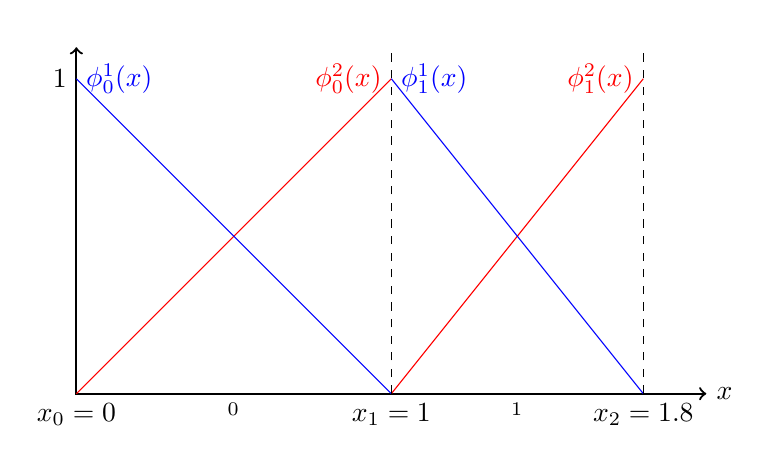
\begin{tikzpicture}[scale=4]
    % Draw axes
    \draw [<->,thick] (0,1.1) node (yaxis) [above] {}
        |- (2,0) node (xaxis) [right] {$x$};
    % Draw two intersecting lines
    \draw[red] (0,0) coordinate (a_1) -- (1,1) coordinate (a_2);
    \draw[blue] (0,1) coordinate (b_1) -- (1,0) coordinate (b_2);
    \draw[red] (1,0) coordinate (a_3) -- (1.8,1) coordinate (a_4);
    \draw[blue] (1,1) coordinate (b_3) -- (1.8,0) coordinate (b_4);
    \draw[dashed] (1,0) coordinate (c_1) -- (1,1.1) coordinate (c_2);
    \draw[dashed] (1.8,0) coordinate (d_1) -- (1.8,1.1) coordinate (d_2);
    \filldraw (0.5,0) circle (0pt) node[align=center, below] {\(\calD_0\)};
    \filldraw (1.4,0) circle (0pt) node[align=center, below] {\(\calD_1\)};
    \filldraw (0,0) circle (0pt) node[align=center, below] {\(x_0=0\)};
    \filldraw (1,0) circle (0pt) node[align=center, below] {\(x_1=1\)};
    \filldraw (1.8,0) circle (0pt) node[align=center, below] {\(x_2=1.8\)};  
    \filldraw (0,1) circle (0pt) node[align=center, left] {\(1\)};    
    \filldraw (0,1) circle (0pt) node[align=center, right] {\color{blue}\(\phi_0^1(x)\)};    
    \filldraw (1,1) circle (0pt) node[align=center, left] {\color{red}\(\phi_0^2(x)\)};    
    \filldraw (1,1) circle (0pt) node[align=center, right] {\color{blue}\(\phi_1^1(x)\)};    
    \filldraw (1.8,1) circle (0pt) node[align=center, left] {\color{red}\(\phi_1^2(x)\)};    
\end{tikzpicture}
\caption{A mesh with nodes \(w_0=0\), \(w_1=1\) and \(w_2=1.8\). There are two basis functions on each cell. Boundaries are located at \(w_0=0\) and \(w_2=1.8\).\label{fig: mesh}}
\end{figure}
We can verify that the matrices \(\bs M\) and \(\bs G\) are given by 
\begin{align*}
	\bs M &= \left[\begin{array}{c|c} \bs M_1 & \bs 0 \\\hline \bs 0 & \bs M_2 \end{array}\right] = \left[\begin{array}{cc|cc} 1/3 & 1/6 & 0 & 0 \\ 1/6 & 1/3 & 0 & 0 \\\hline 0 & 0 & 4/15 & 4/30 \\ 0 & 0 & 4/30 & 4/15 \end{array}\right],
	\\ \bs G &= \left[\begin{array}{c|c} \bs G_1 & \bs 0 \\ \hline \bs 0 & \bs G_2 \end{array}\right] = \left[\begin{array}{cc|cc} -1/2 & 1/2 & 0 & 0 \\ -1/2 & 1/2 & 0 & 0 \\\hline 0 & 0 & -1/2 & 1/2 \\ 0 & 0 & -1/2 & 1/2 \end{array}\right] .
\end{align*}
% The matrix \(\bs P\) is given by 
% \[\bs P = \left[\begin{array}{cc|cc} 1/2 & 0 & 0 & 0 \\ 0 & 1/2 & 0 & 0 \\\hline 0 & 0 & 2/5 & 0 \\ 0 & 0 & 0 & 2/5 \end{array}\right].\]

Let \(c_1=1\) and \(c_2=-2\). Then the cells are \(\mathcal D_{0,1} = (0,1),\,\mathcal D_{1,1}=[1,1.8),\, \mathcal D_{0,2}=(0,1],\, \mathcal D_{1,2}=(1,1.8)\) and the flux matrices are given by 
\begin{align*}
	\bs F_1 &= \left[\begin{array}{c|c} \bs F_1^{00} & \bs F_1^{01} \\\hline \bs 0 & \bs F_1^{11} \end{array}\right] = \left[\begin{array}{cc|cc} 0 & 0 & 0 & 0 \\ 0 & -1 & 1 & 0 \\\hline 0 & 0 & 0 & 0 \\ 0 & 0 & 0 & -1 \end{array}\right],
	\\\bs F_2 &= \left[\begin{array}{c|c} \bs F_2^{00} & \bs 0 \\\hline \bs  F_2^{10} & \bs F_2^{11} \end{array}\right] = \left[\begin{array}{cc|cc} -1 & 0 & 0 & 0 \\ 0 & 0 & 0 & 0 \\\hline 0 & 1 & -1 & 0 \\ 0 & 0 & 0 & 0 \end{array}\right].
\end{align*}

Suppose that \(r_1(x)>0\) on \(\calD_{0,1}=\mathcal F_1^+\) and \(r_1(x)<0\) on \(\calD_{1,1}\cup\{1.8\}=\mathcal F_1^-\), and further, that \(r_2(x)<0\) on \(\{0\}\cup\calD_{0,2}=\mathcal F_2^-\) and \(r_2(x)>0\) on \(\calD_{1,2}=\mathcal F_2^+\). Specifically, let 
\[r_1(x) = \begin{cases} 1 & x \in (0,1), \\ -1 & x \in [1,1.8],\end{cases}\quad r_2(x) = \begin{cases} -1 & x = 0, \\ -2 & x \in (0,1], \\ 1 & x \in (1,1.8). \end{cases}\]

%Therefore, on the interior of the space we have 
%\begin{align*}
%  B &= \left[\begin{array}{cc|cc|cc|cc} 
%T_{11}/3 & T_{11}/6 & 0 & 0 & T_{12}/3 & T_{12}/6 & 0 & 0 \\
%T_{11}/6 & T_{11}/3 & 0 & 0 & T_{12}/6 & T_{12}/3 & 0 & 0 \\\hline 
%0 & 0 & T_{11}/15 & T_{11}/30 & 0 & 0 & T_{12}/15 & T_{12}/30 \\ 
%0 & 0 & T_{11}/30 & T_{11}/15 & 0 & 0 & T_{12}/30 & T_{12}/15 \\\hline
%T_{21}/3 & T_{21}/6 & 0 & 0 & T_{22}/3 & T_{22}/6 & 0 & 0 \\
%T_{21}/6 & T_{21}/3 & 0 & 0 & T_{22}/6 & T_{22}/3 & 0 & 0 \\\hline
%0 & 0 & T_{21}/15 & T_{21}/30 & 0 & 0 & T_{22}/15 & T_{22}/30 \\
%0 & 0 & T_{21}/30 & T_{21}/15 & 0 & 0 & T_{22}/30 & T_{22}/15 
%\end{array}\right] 
%\\&{}+\left[\begin{array}{cc|cc|cc|cc} 
%-1/2 & 1/2 & 0 & 0 & 0 & 0 & 0 & 0 \\
%-1/2 & -1/2 & 1 & 0 & 0 & 0 & 0 & 0 \\\hline 
%0 & 0 & -1/2 & 1/2 & 0 & 0 & 0 & 0 \\ 
%0 & 0 & -1/2 & -1/2 & 0 & 0 & 0 & 0 \\\hline
%0 & 0 & 0 & 0 & -1 & -1 & 0 & 0 \\
%0 & 0 & 0 & 0 & 1 & -1 & 0 & 0 \\\hline
%0 & 0 & 0 & 0 & 0 & 2 & -1 & -1 \\
%0 & 0 & 0 & 0 & 0 & 0 & 1 & -1 
%\end{array}\right].
%\end{align*}
%Reordering and adding the boundary conditions gives 
%\begin{align*}
%\widehat{\mathfrak B} &= \left[\begin{array}{c|cc|cc|cc|cc|c} 
%T_{22} & T_{21} & 0 & 0 & 0 & 0 & 0 & 0 & 0 & 0\\\hline 
%0 & T_{11}/3 & T_{11}/6 & T_{12}/3 & T_{12}/6 & 0 & 0 & 0 & 0 & 0 \\
%0 & T_{11}/6 & T_{11}/3 & T_{12}/6 & T_{12}/3 & 0 & 0 & 0 & 0 & 0 \\\hline 
%0 & T_{21}/3 & T_{21}/6 & T_{22}/3 & T_{22}/6 & 0 & 0 & 0 & 0 & 0 \\ 
%0 & T_{21}/6 & T_{21}/3 & T_{22}/6 & T_{22}/3 & 0 & 0 & 0 & 0 & 0\\\hline
%0 & 0 & 0 & 0 & 0 & T_{11}/15 & T_{11}/30 & T_{12}/15 & T_{12}/30 & 0 \\ 
%0 & 0 & 0 & 0 & 0 & T_{11}/30 & T_{11}/15 & T_{12}/30 & T_{12}/15 & 0\\\hline
%0 & 0 & 0 & 0 & 0 & T_{21}/15 & T_{21}/30 & T_{22}/15 & T_{22}/30 & 0 \\
%0 & 0 & 0 & 0 & 0 & T_{21}/30 & T_{21}/15 & T_{22}/30 & T_{22}/15 & 0 \\\hline
%0 & 0 & 0 & 0 & 0 & 0 & 0 & 0 & T_{12} & T_{11}
%\end{array}\right] 
%\\&{}+\left[\begin{array}{c|cc|cc|cc|cc|c} 
%0 & 0 & 0 & 0 & 0 & 0 & 0 & 0 & 0 & 0\\\hline 
%0 & -1/2 & 1/2 & 0 & 0 & 0 & 0 & 0 & 0 & 0 \\
%0 & -1/2 & -1/2 & 0 & 0 & 1 & 0 & 0 & 0 & 0 \\\hline 
%2 & 0 & 0 & -1 & -1 & 0 & 0 & 0 & 0 & 0 \\ 
%0 & 0 & 0 & 1 & -1 & 0 & 0 & 0 & 0 & 0 \\\hline
%0 & 0 & 0 & 0 & 0 & -1/2 & 1/2 & 0 & 0 & 0 \\
%0 & 0 & 0 & 0 & 0 & -1/2 & -1/2 & 0 & 0 & 1 \\\hline
%0 & 0 & 0 & 0 & 2 & 0 & 0 & -1 & -1 & 0 \\
%0 & 0 & 0 & 0 & 0 & 0 & 0 & 1 & -1 & 0 \\
%0 & 0 & 0 & 0 & 0 & 0 & 0 & 0 & 0 & 0 
%\end{array}\right].
%\end{align*}

Then, constructing \({  \bs B}\) we get 
\begin{center}
\[
\begin{blockarray}{c|cc|cc|cc|cc|c}
{-1} & \BAmulticolumn{4}{c|}{\calD_0} & \BAmulticolumn{4}{c|}{\calD_2} & {K+1}\\
\calF_2^- & \BAmulticolumn{2}{c|}{\calF_1^+} & \BAmulticolumn{2}{c|}{\calF_2^-} & \BAmulticolumn{2}{c|}{\calF_1^-} & \BAmulticolumn{2}{c|}{\calF_2^+} & \calF_1^-\\
q_{{-1},0} & a_{0,1}^1 & a_{0,1}^2 & a_{0,2}^1 & a_{0,2}^2 & a_{1,1}^1 & a_{1,1}^2 & a_{1,2}^1 & a_{1,2}^2 & q_{{K+1},1}\\\BAhline
\begin{block}{[c|cc|cc|cc|cc|c]} 
T_{22} & 4T_{21} & -2T_{21} & 0 & 0 & 0 & 0 & 0 & 0 & 0\\\BAhline
0 & T_{11}-3 & 3 & T_{12} & 0 & 0 & 0 & 0 & 0 & 0 \\
0 & -1 & T_{11}-1 & 0 & T_{12} & 5 & -2.5 & 0 & 0 & 0 \\\BAhline 
2 & T_{21} & 0 & T_{22}-2 & -2 & 0 & 0 & 0 & 0 & 0 \\ 
0 & 0 & T_{21} & 6 & T_{22}-6 & 0 & 0 & 0 & 0 & 0\\\BAhline
0 & 0 & 0 & 0 & 0 & T_{11}-\frac{15}{4} & \frac{15}{4} & T_{12} & 0 & 0 \\ 
0 & 0 & 0 & 0 & 0 & -\frac{5}{4} & T_{11}-\frac{5}{4} & 0 & T_{12} &1\\\BAhline
0 & 0 & 0 & -4 & 8 & T_{21} & 0 & T_{22}-\frac{5}{2} & -\frac{5}{2} & 0 \\
0 & 0 & 0 & 0 & 0 & 0 & T_{21} & \frac{15}{2} & T_{22}-\frac{15}{2} & 0 \\\BAhline
0 & 0 & 0 & 0 & 0 & 0 & 0 & -2T_{12} & 4T_{12} & T_{11} \\
\end{block}
\end{blockarray}.
%\\&{}+\left[\begin{array}{c|cc|cc|cc|cc|c} 
%0 & 0 & 0 & 0 & 0 & 0 & 0 & 0 & 0 & 0\\\hline 
%0 & -3 & 3 & 0 & 0 & 0 & 0 & 0 & 0 & 0 \\
%0 & -1 & -1 & 0 & 0 & 4 & -2 & 0 & 0 & 0 \\\hline 
%4 & 0 & 0 & -2 & -2 & 0 & 0 & 0 & 0 & 0 \\ 
%0 & 0 & 0 & 6 & -6 & 0 & 0 & 0 & 0 & 0 \\\hline
%0 & 0 & 0 & 0 & 0 & -3.75 & 3.75 & 0 & 0 & 0 \\
%0 & 0 & 0 & 0 & 0 & -1.25 & -1.25 & 0 & 0 & 2.5 \\\hline
%0 & 0 & 0 & -5 & 10 & 0 & 0 & -2.5 & -2.5 & 0 \\
%0 & 0 & 0 & 0 & 0 & 0 & 0 & 7.5 & -7.5 & 0 \\\hline
%0 & 0 & 0 & 0 & 0 & 0 & 0 & 0 & 0 & 0 
%\end{array}\right].
\]
\end{center}

We also have sub-matrices
\begin{align*}
	&{  \bs B}_{11}^{++} = \left[\begin{array}{cc}
		T_{11}-3 & 3 \\
		-1 & T_{11}-1
	\end{array}\right],
	\,
	{  \bs B}_{11}^{+-} = \left[\begin{array}{cc|c}
		0 & 0 & 0\\
		5 & -2.5 & 0
	\end{array}\right], 
	%
%	\\&{  B}_{11}^{-+} = \left[\begin{array}{cc}
%		0 & 0 \\
%		0 & 0 \\ \hline
%		0 & 0 
%	\end{array}\right], 
	\,
	\\&{  \bs B}_{11}^{--} = \left[\begin{array}{cc|c}
		T_{11}-\frac{15}{2} & \frac{15}{2} & 0\\
		-\frac{5}{2} & T_{11}-\frac{5}{2} & 1\\\hline
		0 & 0 & T_{11}
	\end{array}\right],
	%%%%%%%%%%%%%%%%%%%
	%%%%%%%%%%%%%%%%%%%
%	\\&{  B}_{12}^{++} = \left[\begin{array}{cc}
%		0 & 0 \\
%		0 & 0 
%	\end{array}\right],
%	\,
	{  \bs B}_{12}^{+-} = \left[\begin{array}{c|cc}
		0 & T_{12} & 0 \\
		0 & 0 & T_{12}
	\end{array}\right], \,
	%
	\\&{  \bs B}_{12}^{-+} = \left[\begin{array}{cc}
		T_{12} & 0 \\
		0 & T_{12} \\\hline
		-2T_{12} & 4T_{12}
	\end{array}\right],
	\, 
%	{  B}_{12}^{--} = \left[\begin{array}{c|cc}
%		0 & 0 & 0 \\
%		0 & 0 & 0
%	\end{array}\right],
	%%%%%%%%%%%%%%%%%%%
	%%%%%%%%%%%%%%%%%%%
	%%%%%%%%%%%%%%%%%%%
%	\\&{  B}_{21}^{++} = \left[\begin{array}{cc}
%		0 & 0 \\
%		0 & 0
%	\end{array}\right],
%	\,
	{  \bs B}_{21}^{+-} = \left[\begin{array}{cc|c}
		T_{21} & 0 & 0 \\
		0 & T_{21} & 0 
	\end{array}\right], \,
	%
	\\&{  \bs B}_{21}^{-+} = \left[\begin{array}{cc}
		4T_{21} & -2T_{21} \\ \hline
		T_{21} & 0 \\
		0 & T_{21} 
	\end{array}\right],
	\, 
%	{  B}_{21}^{--} = \left[\begin{array}{cc|c}
%		0 & 0 & 0 \\\hline
%		0 & 0 & 0 \\ 
%		0 & 0 & 0 
%	\end{array}\right],
	%%%%%%%%%%%%%%%%%%%%
	%%%%%%%%%%%%%%%%%%%%
	{  \bs B}_{22}^{++} = \left[\begin{array}{cc}
		T_{22}-\frac{5}{2} & -\frac{5}{2} \\
		\frac{15}{2} & T_{22} -\frac{15}{2}
	\end{array}\right],
	\,
	\\&{  \bs B}_{22}^{+-} = \left[\begin{array}{c|cc}
		0 & -4 & 8 \\
		0 & 0 & 0 
	\end{array}\right], \,
	%
%	\\&{  B}_{22}^{-+} = \left[\begin{array}{cc}
%		0 & 0 \\\hline
%		0 & 0 \\
%		0 & 0 
%	\end{array}\right], 
%	\,
	{  \bs B}_{22}^{--} = \left[\begin{array}{c|cc}
		T_{22} & 0 & 0\\\hline
		2 & T_{22}-2 & -2\\
		0 & 6 & T_{22}-6
	\end{array}\right],
	%%%%%%%%%%%%%%%%%%%
	%%%%%%%%%%%%%%%%%%%
\end{align*}
and \({  \bs B}_{11}^{-+} = \bs 0_{3\times2},\, {  \bs B}_{12}^{++} = \bs 0_{2\times2},\, {  \bs B}_{12}^{--} = \bs 0_{2\times3},\, {  \bs B}_{21}^{++} = \bs 0_{2\times 2},\, {  \bs B}_{21}^{--} = \bs 0_{3\times3},\, {  \bs B}_{22}^{-+} = \bs 0_{3\times2},\) where \(\bs 0_{n\times m}\) denotes an \(n\times m\) matrix of zeros. Furthermore, 
\begin{align*}
	{  \bs B}^{++} &= \left[\begin{array}{cc|cc}
		T_{11}-3 & 3 & 0 & 0 \\
		-1 & T_{11}-1 & 0 & 0 \\\hline
		0 & 0 & T_{22}-\frac{5}{2} & -\frac{5}{2}\\
		0 & 0 & \frac{15}{2} & -\frac{15}{2}
	\end{array}\right],
	\\
	{  \bs B}^{+-} &= \left[\begin{array}{c|cc|cc|c}
		0 & T_{12} & 0 & 0 & 0 & 0\\
		0 & 0 & T_{12} & 5 & -2.5 & 0\\\hline 
		0 & -4 & 8 & T_{21} & 0 & 0 \\
		0 & 0 & 0 & 0 & T_{21} & 0 
	\end{array}\right], 
	\\
	{  \bs B}^{-+} &= \left[\begin{array}{cc|cc}
		4T_{21} & -2T_{21} & 0 & 0 \\\hline
		T_{21} & 0 & 0 & 0\\
		0 & T_{21} & 0 & 0 \\\hline
		0 & 0 & T_{12} & 0 \\ 
		0 & 0 & 0 & T_{12} \\\hline
		0 & 0 & -2T_{12} & 4T_{12}
	\end{array}\right],
	\intertext{}
	{  \bs B}^{--} &= \left[\begin{array}{c|cc|cc|c}
		T_{22} & 0 & 0 & 0 & 0 & 0 \\\hline 
		2 & T_{22}-2 & -2 & 0 & 0 & 0 \\
		0 & 6 & T_{22}-6 & 0 & 0 & 0 \\\hline 
		0 & 0 & 0 & T_{11}-\frac{15}{4} & -\frac{15}{4} & 0 \\
		0 & 0 & 0 & -\frac{5}{4} & T_{11}-\frac{5}{4} & 1 \\\hline 
		0 & 0 & 0 & 0 & 0 & T_{11}
	\end{array}\right].
\end{align*}

Since \(r_1(x)\) and \(r_2(x)\) are constant on each cell then \(  \bs R^+\) and \(  \bs R^-\) take a particularly simple form. We have 
\[  \bs R^+ = \left[\begin{array}{cc|cc}1&0&0&0\\0&1&0&0\\\hline0&0&1&0\\0&0&0&1\end{array}\right], \quad   \bs R^- = \left[\begin{array}{c|cc|cc|c}1&0&0&0&0&0\\\hline0&1/2&0&0&0&0\\0&0&1/2&0&0&0\\\hline0&0&0&1&0&0\\0&0&0&0&1&0\\\hline0&0&0&0&0&1\end{array}\right].\]

The DG approximations \(  \bs D^{m n}(s),\, m,n\in\{+,-\}\) can now be constructed as 
\[  \bs D^{m n}(s) = \begin{cases}   \bs R^m\left({  \bs B}^{mm} - s \bs I\right) & n=m,
	\\   \bs R^m {  \bs B}^{mn} & n \neq m. \end{cases}\]

For a given value of \(s\), we construct and solve the matrix Riccati equation,
\begin{align*}
	\bs D^{+-}(s)
+ \bs \Psi(s)   \bs D^{-+}(s)\Psi(s)
+   \bs D^{++}(s)\bs \Psi(s)
+ \bs \Psi(s)  \bs D^{--}(s)
= \bs 0,
\end{align*}
for the matrix \(\bs \Psi(s)\) using, for example, Newtons method \citep{bot08}. To obtain the stationary distribution we require \(\bs \Psi(0)\). 

Now, to find \( {\bs\xi}\), we solve the linear system in Equations \eqref{eqn:xi1}-\eqref{eqn:xi2}. The result is a vector which we denote, 
\[ {\bs\xi} = \left[\begin{array}{c|cc|cc|c} {\xi}_{-1,2} &  {\xi}_{0,2}^1 &  {\xi}_{0,2}^2 &  {\xi}_{1,1}^1 &  {\xi}_{1,1}^2 &  {\xi}_{K+1,1} \end{array}\right],\]
where \( {\xi}_{-1,2}\) is an approximation to \( \lim\limits_{n\to\infty}\mathbb{P}\left( X{(\theta_n)} =0, \varphi({\theta_n}) = 2\right)\) and \( {\xi}_{K+1,1}\) is an approximation to the artificial point mass \( \lim\limits_{n\to\infty}\mathbb{P}\left( X({\theta_n}) =1.8, \varphi({\theta_n}) = 1\right)\). For \(x\in\calD_{0,2}\) an approximation to the density of \( \lim\limits_{n\to\infty}\mathbb{P}\left( X({\theta_n}) \in \wrt x, \varphi({\theta_n}) = 2\right)\), is constructed as \( {\xi}_{0,2}^0\phi_0^1(x) +  {\xi}_{0,2}^0\phi_0^1(x)\). For \(x\in\calD_{1,1}\) an approximation to the density of \( \lim\limits_{n\to\infty}\mathbb{P}\left(X({\theta_n}) \in \wrt x, \varphi({\theta_n}) = 1\right)\), is constructed as \( {\xi}_{1,1}^1\phi_1^1(x) +  {\xi}_{1,1}^2\phi_1^2(x).\)

Next, given a value of \(w\), we solve the system \eqref{eqn:pisystem1}-\eqref{eqn:pisystem2} to find \( {\bs p}= {\bs p}^-\) and \( {\bs \pi}(w)\). 

For the point masses we have 
\[ {\bs p}^- = \left[\begin{array}{c|cc|cc|c} {p}_{-1,2} &  {p}_{0,2}^1 &  {p}_{0,2}^2 &  {p}_{1,1}^1 &  {p}_{1,1}^2 &  {p}_{K+1,1} \end{array}\right],\]
where \( {p}_{-1,2}\) is an approximation to \( \lim\limits_{t\to\infty}\mathbb{P}\left(\dot W(t)=0,X({t}) =0, \varphi_{t} = 2\right)\) and \( {p}_{K+1,1}\) is an approximation to the artificial point mass \( \lim\limits_{t\to\infty}\mathbb{P}\left(\dot W(t)=0, X(t) =1.8, \varphi({t}) = 1\right)\). For \(x\in\calD_{0,2}\), an approximation to the density of \( \lim\limits_{t\to\infty}\mathbb{P}\left( \dot W(t)=0, X(t) \in \wrt x, \varphi({t}) = 2\right)\), is constructed as \( {p}_{0,2}^1\phi_0^1(x) +  {p}_{0,2}^2\phi_0^2(x)\). For \(x\in\calD_{1,1}\), an approximation to the density of \( \lim\limits_{t\to\infty}\mathbb{P}\left(\dot W(t)=0, X(t) \in \wrt x, \varphi({t}) = 1\right)\), is constructed as \( {p}_{1,1}^1\phi_1^1(x) +  {p}_{1,1}^2\phi_1^2(x).\)

Similarly, for \( {\bs\pi}^-(w)\), we have 
\[ {\bs \pi}^-(w) = \left[\begin{array}{c|cc|cc|c} {\pi}_{-1,2}(w) &  {\pi}_{0,2}^1(w) &  {\pi}_{0,2}^2(w) &  {\pi}_{1,1}^1(w) &  {\pi}_{1,1}^2(w) &  {\pi}_{K+1,1}(w) \end{array}\right],\]
where \( {\pi}_{-1,2}(w)\) is an approximation to \( \lim\limits_{t\to\infty}\mathbb{P}\left(  \dot W(t)\in\wrt w, X(t) =0, \varphi({t}) = 2\right)\) and \( {\pi}_{K+1,1}(w)\) is an approximation to the artificial point mass \( \lim\limits_{t\to\infty}\mathbb{P}\left( \dot W(t)\in \wrt w, X(t) =1.8, \varphi({t}) = 1\right)\). For \(x\in\calD_{0,2}\) an approximation to the density of \( \lim\limits_{t\to\infty}\mathbb{P}\left(\dot W(t) \in \wrt w, X(t) \in \wrt x, \varphi({t}) = 2\right)\), is constructed as \( {\pi}_{0,2}^1(w)\phi_0^1(x) +  {\pi}_{0,2}^2(w)\phi_0^2(x)\). For \(x\in\calD_{1,1}\) an approximation to the density of \( \lim\limits_{t\to\infty}\mathbb{P}\left( \dot W(t) \in \wrt w, X(t) \in \wrt x, \varphi({t}) = 1\right)\), is constructed as \( {\pi}_{1,1}^1(w)\phi_1^1(x) +  {\pi}_{1,1}^2(w)\phi_1^2(x).\)

For \( {\bs\pi}^+(w)\), we have 
\[ {\bs \pi}^+(w) = \left[\begin{array}{cc|cc}  {\pi}_{0,1}^1(w) &  {\pi}_{0,1}^2(w) &  {\pi}_{1,2}^1(w) &  {\pi}_{1,2}^2(w) \end{array}\right].\]
For \(x\in\calD_{0,1}\) an approximation to the joint density of \( \lim\limits_{t\to\infty}\mathbb{P}\left(\dot W(t) \in \wrt w, X_t \in \wrt x, \varphi({t}) = 1\right)\) is constructed as \( {\pi}_{0,1}^1(w)\phi_0^1(x) +  {\pi}_{0,1}^2(w)\phi_0^2(x)\). For \(x\in\calD_{1,2}\) an approximation to the density of \( \lim\limits_{t\to\infty}\mathbb{P}\left(\dot W(t) \in \wrt w,  X(t) \in \wrt x, \varphi({t}) = 2\right)\) is constructed as \( {\pi}_{1,2}^1(w)\phi_1^1(x) +  {\pi}_{1,2}^2(w)\phi_1^2(x).\)

In summary, for \(i\in\calS\), a global approximation of the joint stationary distribution is
\begin{align*}
	\lim\limits_{t\to\infty}\mathbb{P}\left(\dot W(t) \in \wrt w,  X(t) \in \wrt x, \varphi({t}) = i\right) &\approx \displaystyle \sum_{r\in\{1,2\},k\in\{0,1\}}  {\pi}_{i,k}^r(w)\phi_k^r(x)\wrt x \wrt w ,\intertext{ for \(x\in(0,1.8),\, w>0, and\)}
	\lim\limits_{t\to\infty}\mathbb{P}\left( \dot W(t)=0, X(t) \in \wrt x, \varphi({t}) = i\right) & \approx \displaystyle \sum_{r\in\{1,2\},k\in\{0,1\}}  {p}_{k,i}^r\phi_k^r(x)\wrt x ,\quad x\in(0,1.8),\\
	 \lim\limits_{t\to\infty}\mathbb{P}\left(\dot W(t) \in \wrt w,X(t) =0 ,\varphi({t}) = i\right) & \approx{\pi}_{-1,i}(w)\wrt w,\quad w>0, \\
	 \lim\limits_{t\to\infty}\mathbb{P}\left( \dot W(t) =0, X(t) =0,\varphi({t}) = i\right) & \approx {p}_{-1,i},\quad \\ 
	 \lim\limits_{t\to\infty}\mathbb{P}\left(  \dot W(t) \in \wrt w, X(t) = 1.8, \varphi({t}) = i\right) & \approx {\pi}_{K+1,i}(w)\wrt w,\quad w>0, \\
	 \lim\limits_{t\to\infty}\mathbb{P}\left( \dot W(t) = 0, X(t) = 1.8, \varphi({t}) = i\right) & \approx {p}_{K+1,i}.\quad
\end{align*}
%\[\left[\begin{array}{c|cc|cc|cc|cc|c} {\pi}_{2,{-1}}(w) &  {\pi}_{1,1}^1(w) &  {\pi}_{1,2}^1(w) &  {\pi}_{2,1}^1(w) &  {\pi}_{2,2}^1(w) &  {\pi}_{1,1}^2(w) &  {\pi}_{1,2}^2(w) &  {\pi}_{2,1}^2(w) &  {\pi}_{2,2}^2(w) &  {\pi}_{1,{K+1}}(w) \end{array}\right]\]